\documentclass[a4paper,10pt]{scrartcl}
\usepackage[margin=2cm,bindingoffset=0cm]{geometry}
\usepackage{ucs}
\usepackage[utf8x]{inputenc}
\usepackage[ngerman]{babel}
\usepackage{fontenc}
%\usepackage[pdftex]{graphicx}
\usepackage{listings}
\usepackage{amssymb}
\usepackage{amsmath}
\usepackage{wasysym}
\usepackage{graphicx}
\usepackage[pdftex]{hyperref}
\author{Verena Käfer (2551188), Niklas Schnelle (2573250), Peter Vollmer (2553704)}
\date{erstellt am 25.10.2010\\
Version: 1.0}
\title{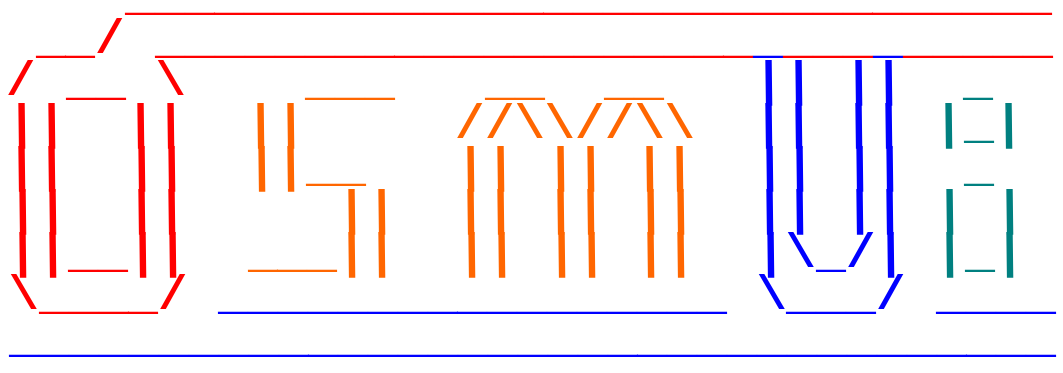
\includegraphics[width=15cm]{Logo_Osmui.png} \\ 
Projektplan von OsmUi}

\begin{document}
\maketitle
\newpage
\tableofcontents
\newpage


\section{Einleitung}
\subsection{Zweck, Abgrenzung}
OsmUi stellt eine benutzerfreundlichere Schnittstelle zur Benutzung von Osmosis dar. Hierbei soll das Pipeline Modell, welches von Osmosis verwendet wird, auf ein leicht benutzbares GUI Modell übertragen werden.
OsmUi verarbeitet selbst keine Daten von OpenStreetMap, sondern generiert Aufrufe für Osmosis. 
\subsection{Projektüberblick, Motivation}
Da es sehr mühselig ist, die komplexen Pipeline-Konstruktionen für Osmosis immer wieder per Hand auf der Kommandozeile oder in einer bat/sh Datei einzugeben, 
entstand die Idee einer grafischen Benutzeroberfläche für Osmosis.
Diese Idee wird nun in Form des Softwarepraktikums im Wintersemester 2010/11 an der Universität Stuttgart umgesetzt.
Eine der so entstehenden Lösungen ist OsmUi, folgende Grundfunktionalitäten sollen durch OsmUi zur Verfügung gestellt werden:
\begin{itemize}
\item Generierung einer Kommandozeile
\item Graphische Aufbereitung der Task-Auswahl und Konstruktion von Pipelines
\end{itemize}

\section{Formale Grundlagen}
\subsection{Vertragliche Anforderungen an die Projektdurchführung}
Das Projekt muss bis zum 01.02.2010 fertiggestellt werden. Dabei werden pro Person 180 Arbeitsstunden veranschlagt.
\subsection{Vertragliche Anforderungen an das Projekt}
\begin{itemize}
\item OsmUi muss mit 100 Tasks gleichzeitig klarkommen und auf allen Plattformen laufen, die Java SE unterstützen.  
\end{itemize}
\section{Leistungen der Vertragspartner}
\subsection{Lieferumfang (Software, Dienstleistungen)}
Im Lieferumfang enthalten sind:
\begin{itemize}
\item OsmUi
\item Handbuch (online / PDF) in englischer Sprache
\item Code
\item Installationsanleitung
\end{itemize}
\subsection{Resultate, die nicht zum Lieferumfang gehören}
Testplan, Projektplan, Spezifikation
\subsection{Leistungen des Auftraggebers}
Leistungen des Auftraggebers:
\begin{itemize}
\item Bibliothek zum Auswählen des Kartenausschnitts.
\item Bibliothek zum Preview der durch Osmosis generierten Ausgabe
\item kleines komplettes Beispiel für eine typische Osmosis Benutzung
\item einige Beispiel-Kommandozeilenaufrufe
\end{itemize}

\subsection{Externe Meilensteine}
\begin{tabular}{|c|c|p{14em}|p{14em}|}
\hline Datum & Uhrzeit & Beschreibung & Meilensteinbeauftragter\\ 
\hline 19.10.2010 & 15:45 - 17:15 Uhr & Kick-Off & Verena Käfer, Niklas Schnelle, Peter Vollmer\\ 
\hline 29.10.2010 & 12:00 Uhr & Abgabe Analysenotizen + Projektplan & Peter Vollmer\\ 
\hline 16.11.20101 & 12:00 Uhr & Abgabe Spezifikation + UI Prototyp & Niklas Schnelle\\ 
\hline 30.11.2010 & 12:00 Uhr & Abgabe korrigierte Spezifikation + Zwischenstand Zeitabrechnung & Verena Käfer\\ 
\hline 14.12.2010 & 12:00 Uhr & Abgabe Entwurf & Peter Vollmer\\ 
\hline 31.12.2010 & 23:59 Uhr & Abgabe Zwischenstand Implementierung (Alpha) + Systemtestplan & Niklas Schnelle\\ 
\hline 11.01.2011 & 12:00 Uhr & Abgabe Implementierung (Beta) + Modultest & Verena Käfer\\ 
\hline 25.01.2011 & 12:00 Uhr & Abgabe Implementierung (RC) + Systemtestprotokoll & Peter Vollmer\\ 
\hline 01.02.2011 & ganzer Tag & Abnahme durch den Kunden & Verena Käfer, Niklas Schnelle, Peter Vollmer\\ 
\hline 11.02.2011 & & Ende des Softwarepraktikums & Verena Käfer, Niklas Schnelle, Peter Vollmer\\ 
\hline 
\end{tabular} 
\subsection{Abnahmeprozedur}
Die Abnahme erfolgt durch den Kunden, vertreten durch Igor Podolskiy und/oder Holger Röder.
\subsection{Änderungsverfahren}
Anforderungsänderungen werden vom Kunde über das Kundenforum bekannt gegeben. Vom Hersteller ausgehende Änderungswünsche werden mit dem
Kunden und den Betreuern abgesprochen.


\section{Entwicklungsprozess}
\subsection{Strategie für die Entwicklung und Integration}
Die Entwicklung erfolgt nach einem erweiterten Wasserfallmodell.
In der Implementierungsphase wird außerdem verstärkt Pair Programming eingesetzt werden.
Hierbei wird die Entwicklung von einem Chief Programmer geleitet, dabei ist wichtig, dass dieser die Verantwortung für die eigentliche Entwicklung trägt.
%\subsection{Projektspezifische Abweichungen vom Standardprozess}

\subsection{Phasen der Entwicklung}
Die weitere Entwicklung erfolgt in  folgenden Phasen:
\begin{enumerate}
\item
Spezifikation und Spezifikationsreview
\item
Entwurf, unter anderem mit UML Diagrammen
\item
Implementierung, sowohl des  eigentlichen Softwaresystems als auch der Unit Tests,
wobei bereits fertige Einheiten so früh wie möglich mit passenden Unit Tests getestet werden.
\item 
Test des Gesamtsystems und Korrektur von Fehlern
\item
Interne Abnahme bei erfolgreich bestandenen Tests des Gesamtsystems
\item
Abnahme durch den Kunden
\end{enumerate}
\subsection{Dokumentationsplan}
Folgende Dokumente werden erstellt und auf dem aktuellen Stand gehalten:
\begin{itemize}
\item Projektplan + Gantt- und Termin-Drift-Diagramm
\item Spezifikation
\item Handbuch/Online-Hilfe
\item Source/API Dokumentation mit Javadoc. Hierbei wird als Teil des Styleguides jede nach außen sichtbare (public) Methode und jede Klasse dokumentiert.
\end{itemize}

\section{Risiken}
\subsection{Risiken und ihre Bewertung}
\begin{itemize}
\item Serverabstürze/Datenverlust\\
Dieses Risiko ist hoch, wobei es meist durch Fehlbedienung und nicht durch Hardwareausfall auftritt.
\item Ausscheiden eines Teilnehmers aus dem Projekt\\
Dieses Risiko ist gering.
\item Temporärer Ausfall eines Teilnehmers aus dem Projekt.\\
Dieses Risiko ist hoch, da Krankheiten nicht vorhergesehen werden können.
\end{itemize}


\subsection{Maßnahmen zur Reduktion der Risiken}
\subsubsection{Datenverlust}
Um dem Verlust wichtiger Projektdaten vorzubeugen, wird Git als dezentralisiertes Versionsverwaltungssystem eingesetzt.
So hat jeder Entwickler immer eine gesamte Kopie der Versionshistorie. Diese kann so von jedem wieder hergestellt werden, sollte sie auf dem Projektserver oder bei einem der Entwickler verloren gehen.
\subsubsection{Wegfall}
Durch sorgfältige Dokumentation und einer detaillierten Spezifikation fällt es neuen Mitarbeitern leichter sich einzuarbeiten.
\subsubsection{Ausfall}
Durch das vermeiden unnötiger Risiken wird temporärer Ausfall minimiert.
\subsection{Notfallpläne}
Im Notfall an den Betreuer wenden.
\section{Richtlinien für die Entwicklung}
\subsection{Konfigurationsmanagement}
Als Konfigurationsverwaltung wird Git verwendet sowie als webbasiertes Projektmanagementtool Trac. Des weiteren existiert eine projektinterne Mailingliste.
\subsection{Design- und Programmierrichtlinien}
Als Programmierrichtlinie wird die Java Code Convention von Oracle/Sun verwendet, siehe \url{http://www.oracle.com/technetwork/java/codeconvtoc-136057.htm}
Als Dokumentationssystem wird Javadoc verwendet.
\subsection{Einsatz von Werkzeugen}
Folgende Werkzeuge werden eingesetzt:
\begin{itemize}
\item GTD-Manager für die Erstellung von Gantt- und Termindriftdiagrammen
\item Visual Paradigm für die UML-Modellierung
\item RevAger zur Review-Organisation
\item Eclipse Helios als IDE
\item Eclipse-Plugin CodeCover zur Coverage Messung
\item Justus zur Testfallverwaltung
\end{itemize}
\section{Anforderungen an die Umgebung}
Die Software wird auf allen durch Java SE unterstützen Systeme lauffähig sein, denn es werden nur reine Java Bibliotheken eingesetzt.
%\subsection{Infrastruktur (Büros, Rechnersysteme, Software)}
%\subsection{Leistungen Dritter im Unternehmen}
%\subsection{Leistungen externer Lieferanten}

\section{Projektorganisation}
\subsection{Schnittstelle zum Auftraggeber}
Schnittstelle zum Kunden ist das Kundenforum. 
\subsection{Schlüsselpersonen}
\begin{itemize}
\item
Projektleiter : Peter Vollmer (vollmepr@studi.informatik.uni-stuttgart.de)
\item
Chiefprogrammer : Niklas Schnelle (schnelns@studi.informatik.uni-stuttgart.de)
\item
Chieftester : Verena Käfer (kaeferva@studi.informatik.uni-stuttgart.de
\item
externer Kunden : Igor Podolskiy\\
(\href{http://www.uni-stuttgart.de/iev/institut/php-Dateien/php_HompageAnzeigen.php?Name=Pd}{http://www.uni-stuttgart.de/iev/institut/php-Dateien/php\_HompageAnzeigen.php?Name=Pd})
\item
interner Kunde : Holger Röder\\
(\href{http://www.iste.uni-stuttgart.de/se/menschen/roeder.html}{http://www.iste.uni-stuttgart.de/se/menschen/roeder.html})
\item 
Betreuer : Daniel Kulesz\\
(\href{http://www.iste.uni-stuttgart.de/se/menschen/kulesz.html}{http://www.iste.uni-stuttgart.de/se/menschen/kulesz.html})
\end{itemize}
\subsection{Organisation}
Da wir als 3 Personen Team eine sehr kleine Gruppe sind treffen sich in aller Regel alle Teammitglieder zum gemeinsamen Arbeiten, dies schafft
kurze Kommunikationswege und ermöglicht es sehr schnell auf Probleme und Fragen zu reagieren. Hierbei ist allerdings darauf zu achten, dass
dabei die Entstehung von Dokumenten nicht behindert wird. Dies wird durch klare Dokumentationsregeln sichergestellt.
Ist direkte Kommunikation gerade nicht möglich wird eine Mailingliste oder ähnliche Kommunikation genutzt. 

\subsubsection{Differentation in den Entwicklungsphasen}
Generell sind in unserem Team alle Mitglieder gleichberechtigt, jedoch liegt die Entscheidungshoheit und Verantwortung in der jeweiligen Phase bei dem dafür Verantwortlichen.
\begin{itemize}
\item In der Planungs-/Analysephase ist der Projektleiter verantwortlicht und trifft bei Uneinigkeit die entgültigen Entscheidungen
\item Da in der Spezifikationsphase die eigentliche Funktionalität und Ausgestaltung der Software beschlossen wird, müssen hier wichtige Entscheidungen
      im Konsens beschossen werden. Betreffen diese einen speziellen Bereich wie die Implementierung kann der hierfür Verantwortliche hóher gewichtet werden.
\item In der Entwurfs- und Implementierungsphase trägt der Chiefprogrammer die Verantwortungen und kann im Streitfall entscheiden
\item In der Testphase entscheidet der Chieftester, er bestimmt auch wann das Testende erreicht ist
\end{itemize}
%\subsection{Berichtwesen}

\section{Entwicklungsplan}
\subsection{Projektstrukturplan (Arbeitsgliederung)}
Das Projekt beinhaltet folgende Arbeitspakete:
\begin{itemize}
\item Projektplan
\item Spezifikation
\item Review der Spezifikation
\item Überarbeitung der Spezifikation nach Review
\item Entwurf
\item Implementierung
\item Modultest
\item Systemtest
\item Handbuch
\item Auslieferung
\item Sonstiges
Mit dem Schreiben des Handbuchs soll möglichst früh nach Fertigstellung der Spezifikation begonnen
werden. Zudem soll das Handbuch in den Projektphasen Entwurf und Implementierung stets mit
den anderen Dokumenten konsistent gehalten und ggf. erweitert werden. Nach Fertigstellung der
Projektphase Implementierung soll das Handbuch noch einmal überarbeitet werden.
Die Modultests sollen direkt vor der Implementierung des zugehörigen Moduls erstellt werden, um
Fehler in der Implementierung frühzeitig erkennen und beheben zu können.
\end{itemize}
\subsection{Terminplan}
\subsubsection{Gantt Diagramm}
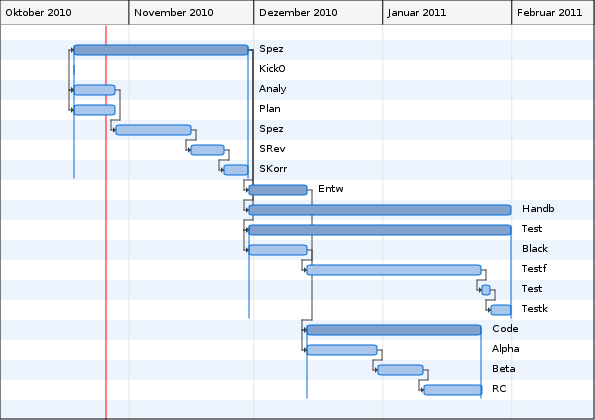
\includegraphics[width=15cm]{gantt.png}
\subsubsection{Termin-Drift Diagramm}
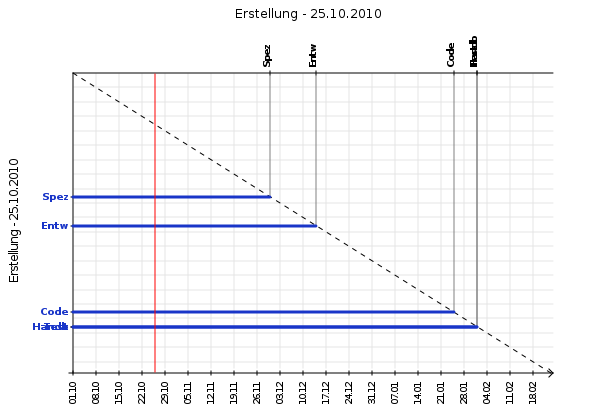
\includegraphics[width=15cm]{termindrift.png}
\subsubsection{Legende}
Entwicklungsphasen:
\begin{itemize}
\item Spez - Analyse und Spezifikation
\item Entw - Entwurf
\item Code - Implementierung
\item Test - Test
\end{itemize}
Untergeordnete Entwicklungsphasen:
\begin{itemize}
\item KickO - Projektbeginn
\item Analy - Erstellung der Analyse, Kundengespräch
\item Plan - Erstellung des Projektplan
\item Spez - Erstellung der Spezifikation
\item SRev - Review der Spezifikation
\item SKorr - Korrektur der Spezifikation anhand des Reviewprotokolls
\item Handb - Erstellung des Handbuchs anhand der Spezifikation und deren Korrektur
\item Black - Erstellung der Blackboxtests anhand der Spezifikation
\item Testf -Erstellung der Modul und Unit-Tests 
\item Test - Testphase mit allen Testfällen
\item Testk - Korrekturphase nach der Testphase
\item Alpha - Zwischenstand mit einigen Grundfunktion der Software
\item Beta - Lauffähige mit allen Grundfuktionen ausgestattete Version mit meist noch bekannten Fehler
\item RC - Lauffähige Version die keine bekannten Fehler mehr. hat und ausgliefert werden soll

\end{itemize}
\subsection{Kostenplan}
Es werden pro Person 180 Arbeitsstunden veranschlagt, dem Kunden entstehen aber keine Kosten.

\end{document}
